\lstinputlisting[language=bash,basicstyle=\small]{python_codes/fieldstone_25/keywords}

This numerical experiment was first presented in \cite{vaks97}.
It consists of an isothermal Rayleigh-Taylor instability in a two-dimensional box
of size $Lx=0.9142$ and $L_y=1$.
Two Newtonian fluids are present in the system: the buoyant layer is placed at the bottom of 
the box and the interface between both fluids is given by 
$
y(x)=0.2+0.02\cos \left( \frac{\pi x}{L_x}  \right)
$
The bottom fluid is parametrised by its mass density $\rho_1$ and its viscosity $\mu_1$, 
while the layer above is parametrised by $\rho_2$ and $\mu_2$.

No-slip boundary conditions are applied at the bottom and at the top of the box 
while free-slip boundary conditions are applied on the sides. 

In the original benchmark the system is run over 2000 units of dimensionless time and the 
timing and position of various upwellings/downwellings is monitored. 
In this present experiment only the root mean square velocity is measured at $t=0$:
the code is indeed not yet foreseen of any algorithm capable of tracking deformation.

Another approach than the ones presented in the extensive literature which showcases 
results of this benchmark is taken. The mesh is initially fitted to the fluids
interface and the resolution is progressively increased. This results in the 
following figure:

\begin{center}
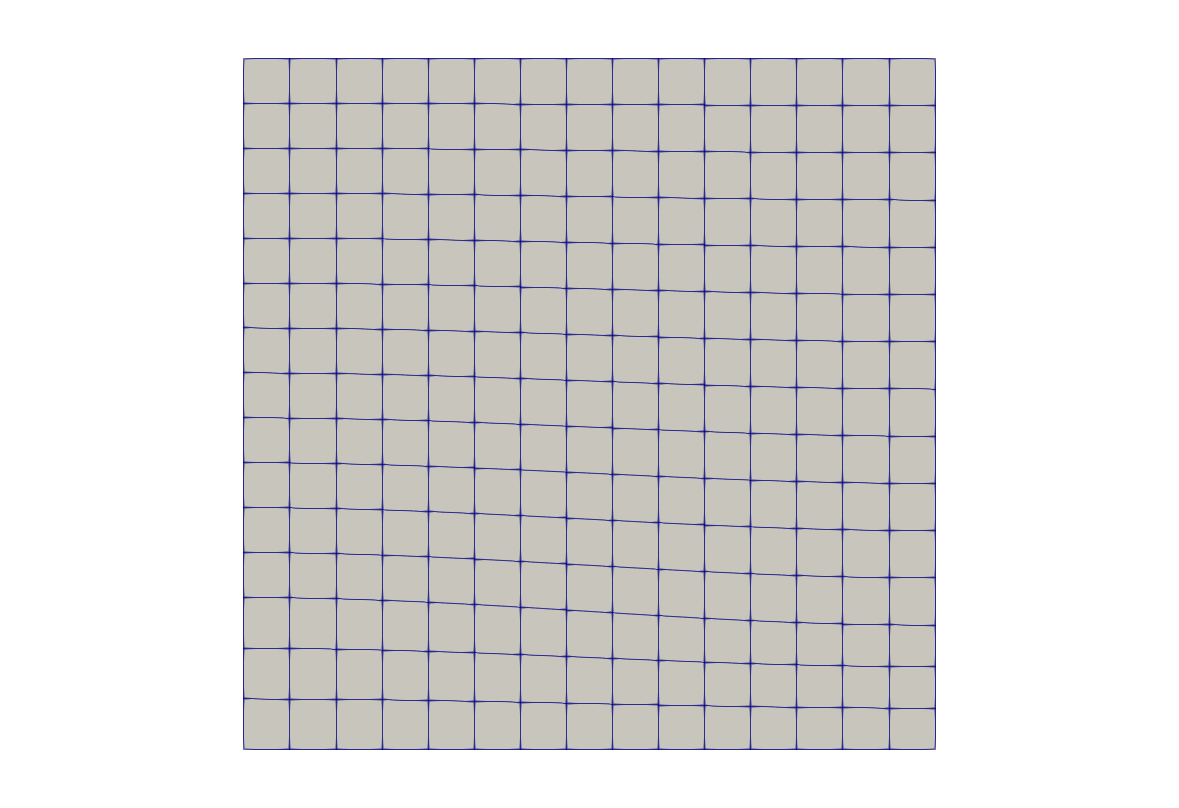
\includegraphics[width=7cm]{python_codes/fieldstone_25/results/grid}
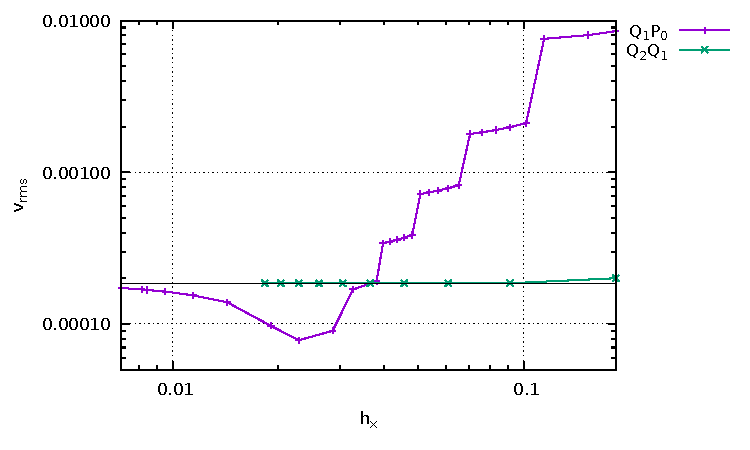
\includegraphics[width=8cm]{python_codes/fieldstone_25/results/vrms.pdf}
\end{center}
The green line indicates results obtained with my code ELEFANT with grids up to 2000x2000
with the exact same methodology.

\begin{center}
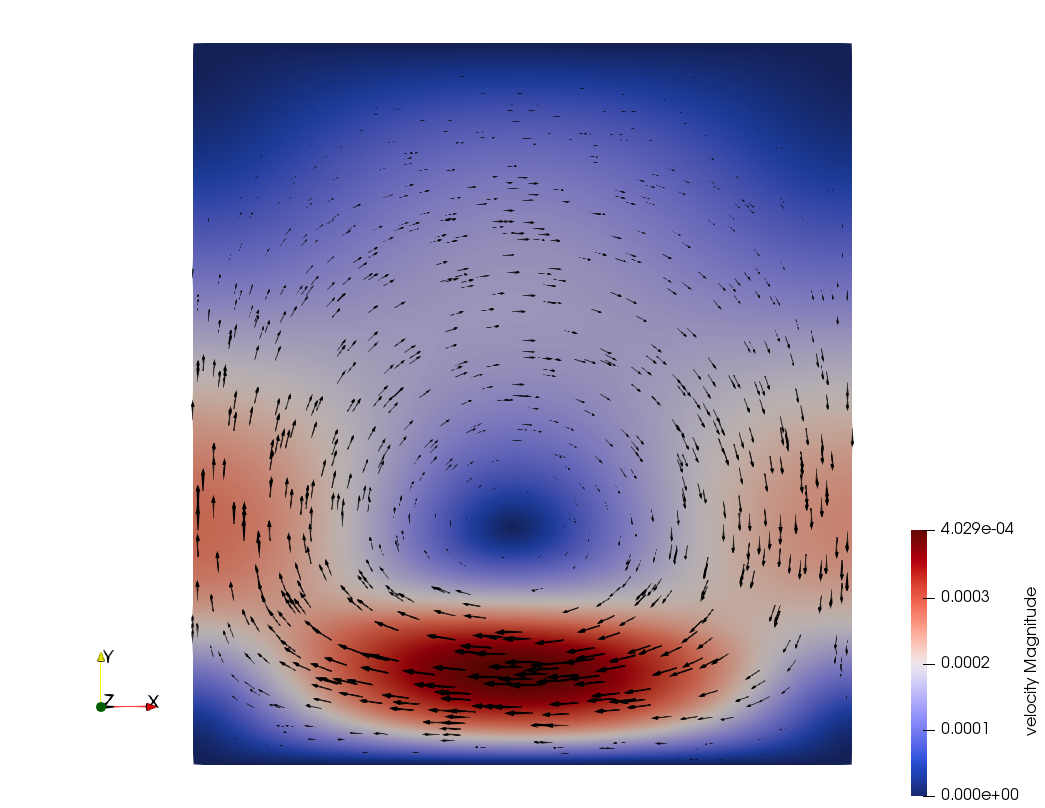
\includegraphics[width=7.5cm]{python_codes/fieldstone_25/results/vel}
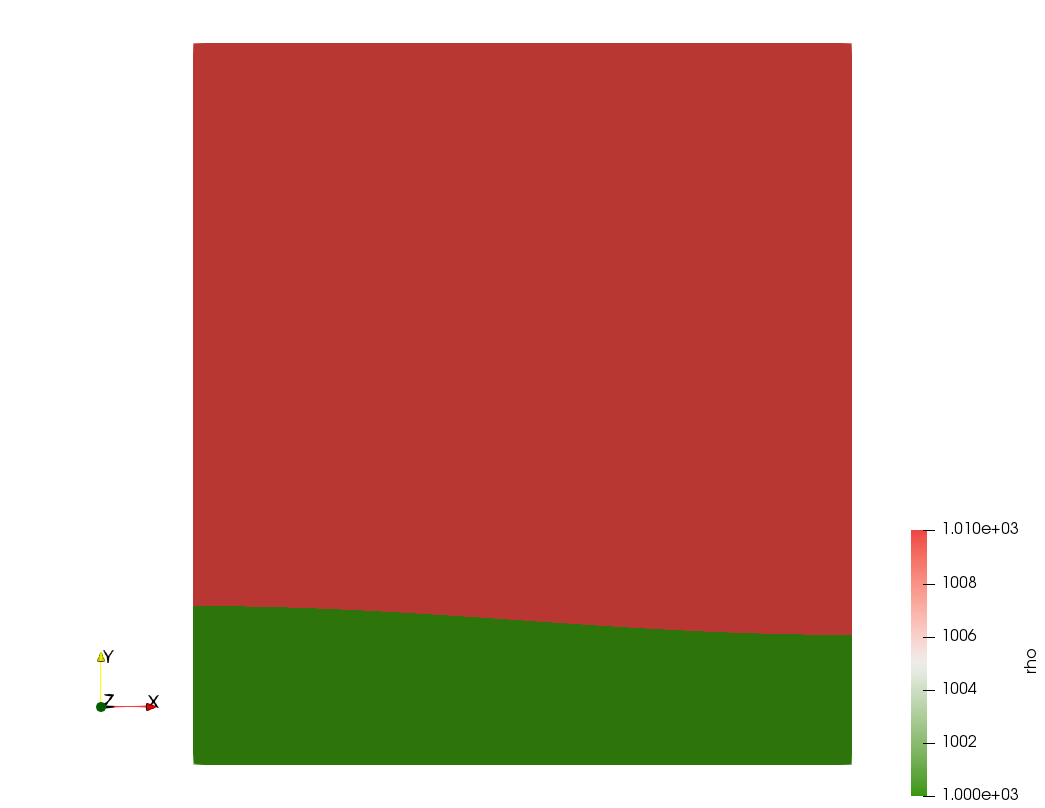
\includegraphics[width=7.5cm]{python_codes/fieldstone_25/results/rho}\\
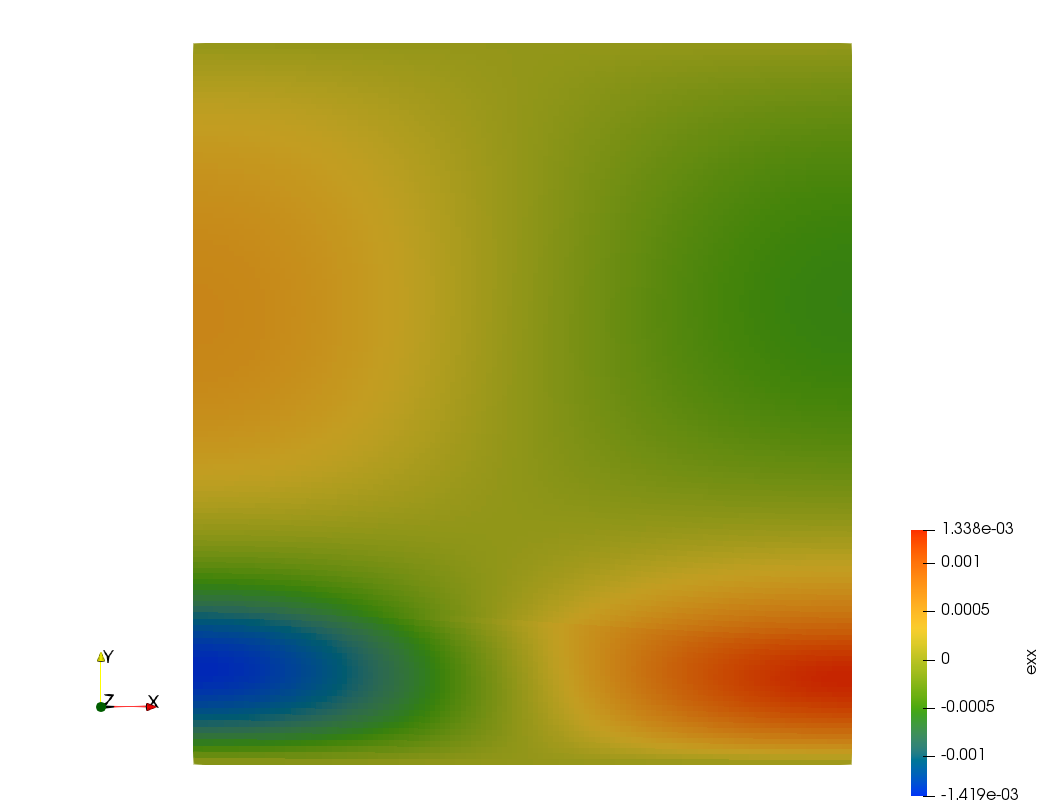
\includegraphics[width=7.5cm]{python_codes/fieldstone_25/results/exx}
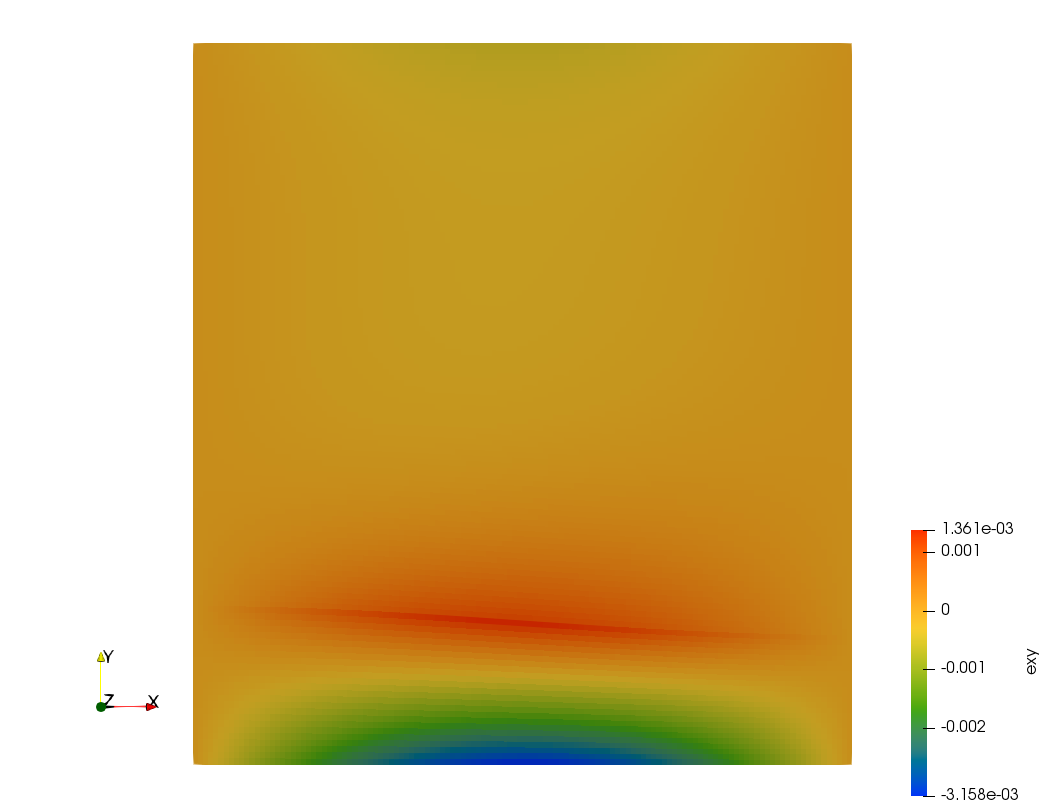
\includegraphics[width=7.5cm]{python_codes/fieldstone_25/results/exy}\\
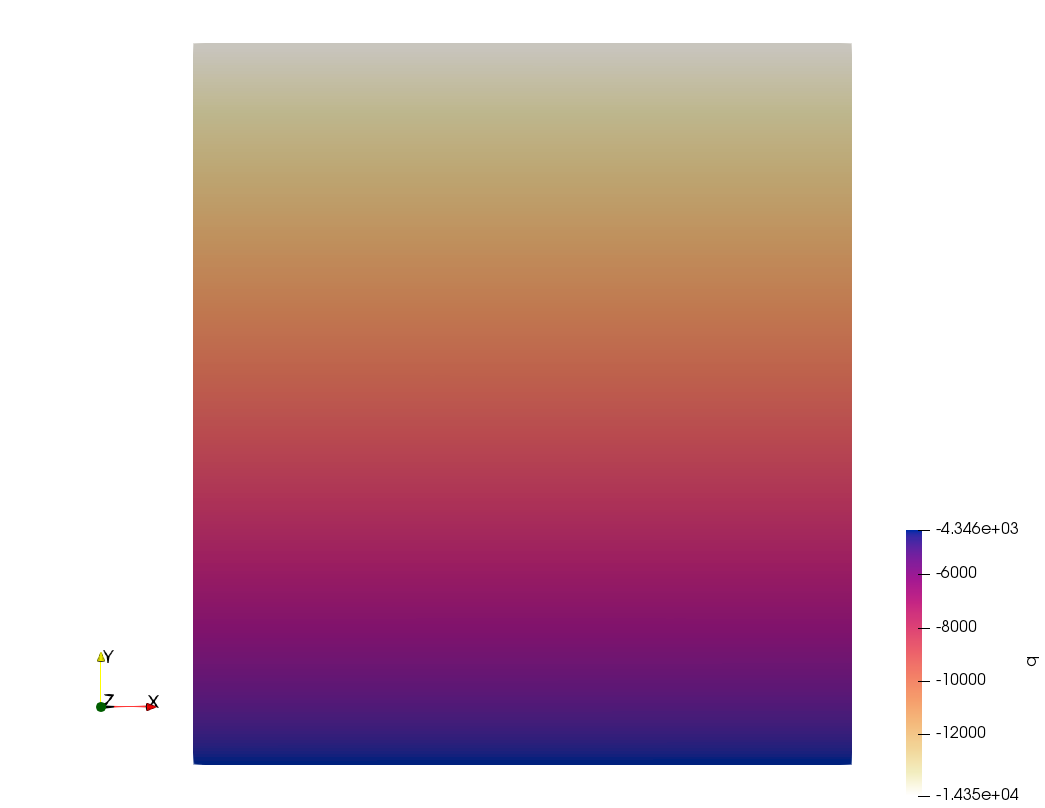
\includegraphics[width=7.5cm]{python_codes/fieldstone_25/results/q}
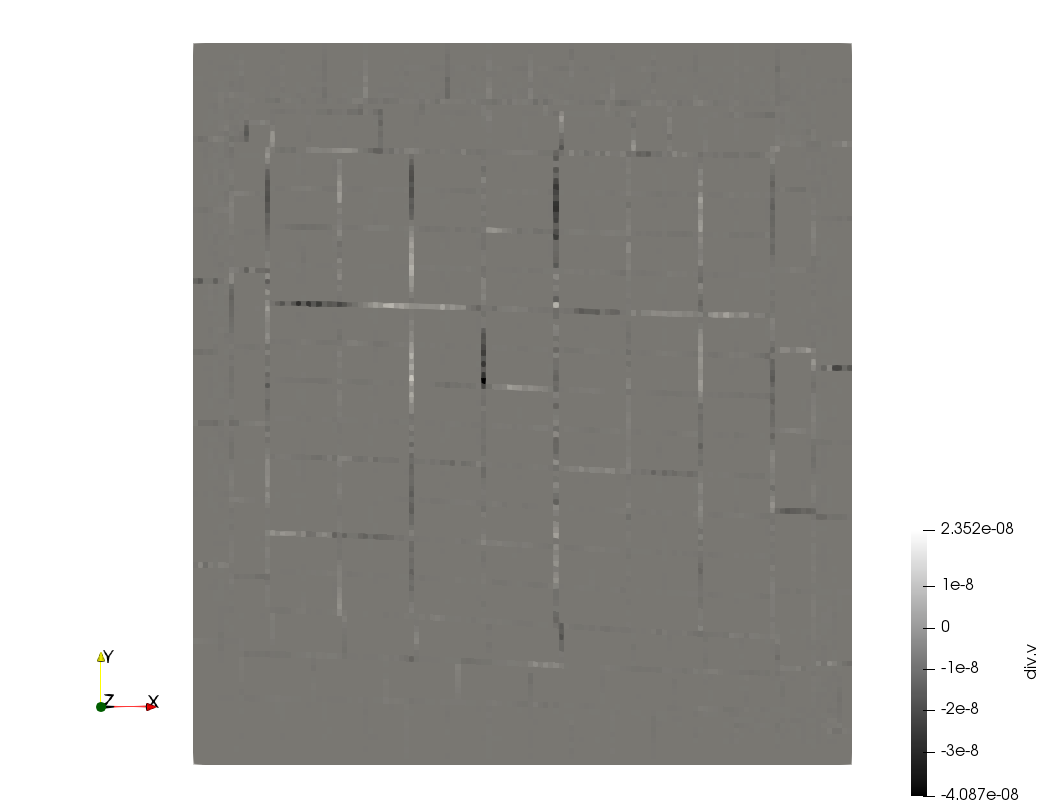
\includegraphics[width=7.5cm]{python_codes/fieldstone_25/results/divv}\\
{\captionfont Results obtained with $Q_1\times P_0$ elements.}
\end{center}








